%-------------------------------------------------------------------------------
\section{Data Disguising}
%-------------------------------------------------------------------------------
%-------------------------------------------------------------------------------
\subsection{Conceptual Model}
%-------------------------------------------------------------------------------

Disguises move a target object along a spectrum from an ``revealed'' 'extreme, in which the target's
identity and correlated data remain intact; to a ``split-up'' extreme, in which objects reachable
from the target are unreachable from any object in the graph. In a split-up state, reachable
objects have either been decorrelated from the target and the rest of the graph by breaking paths in
the graph---or removed entirely.

Subsequent disguises applied to the same target monotonically move the target further
toward the split-up end of the spectrum: application of a disguise can only 
remove or decorrelate reachable objects from the target that prior disguises had not
rendered unreachable.
%objects remain reachable, disguises morph objects

%-------------------------------------------------------------------------------
\subsection{Disguise Specifications}
%-------------------------------------------------------------------------------
Disguise specifications determine how to handle every object reachable from the target (including
the target object itself). An \emph{referencer} object has a (\eg foreign key) reference to another
object. Reachable objects split into one or more guises, each of which is then correlated with some
number of referencers. The original object that has split is removed from the graph:
future disguises to the same target will reach at most the object's guises.

Splitting an object into multiple guises breaks paths between the object and its referencers. 
Referencers of one guise created may not be modified by a future disguise that
reaches another guise of the object. 

If it is impossible to create guises for the object, then the object
and its descendents are recursively removed. (Note that if we do not remove the referencer's
descendents, these have to refer to \emph{something}; if we create guises for the referencers, then
these guises have to refer to something, etc. etc.)

To specify a disguise, the developer writes a set of declarative policies. Each policy describes how
to split objects that satisfy particular predicate conditions, and includes the following:
\begin{enumerate}
    \item Object Type
    \item Predicates: filters out which objects to modify, takes object content as input
    \item Split Spec: how referencers are reallocated between guises
    \item Unique-Guise Spec: how to create a guise that has a unique referencer
    \item Shared-Guise Spec: how to create a guise that ends up with many referencers 
\end{enumerate}

\paragraph{Guise Specifications}
In the following, we assume that objects have identifier attributes (\eg \texttt{id} in
Figure~\ref{fig:guises}); and some attributes are reference attributes that form edges in the graph
to referred objects (\eg \texttt{tag\_id} is a foreign key constraint to tag objects).

Morph specifications are specified at attribute-level granularity. Guise identifier attributes are
unique and random values.  Reference attributes are always copied (handling policies of the
referenced object type will already have decorrelated if necessary).

Other, non-referencing guise attributes either copy the original object's attribute value, or
transform the object's value.  An attribute transformation takes the object attribute value as
input, and generates a new guise value (\eg hashing the value, generating random values, or setting
the value to some default).  The guise attribute value depends at most on the value of the object's
attribute.

The developer writes a guise specification both to create unique guises that are referenced by a single
referencer, and guises that are shared by many referencers.

\paragraph{Split Specification}
The split specification determines, for every type of referencer object, whether referencers of that
type should either (1) be removed (along with its descendents), (2) reference a unique guise and be
the only object with a reference to that guise, or (3) reference a shared guise. 

A split specification includes a set of split policies. Each policy specifies the referencer object
type, a set of predicates to choose the  applicable objects, and a choice to either remove these
objects, or split these objects to reference a unique guise or a shared guise.
There can be more than one policy for a referencer object type: for example, perhaps only
referencer papers over two years old should be removed, while the other papers should be split off
to reference a unique guise.

If any referencers do not fall under any specific split policy in the split specification, they will
all reference a ``global'' shared guise; multiple types of referencers may thus share references to
this global guise.

Split policies are applied with the following precedence:
\begin{enumerate}
    \item Objects are removed
    \item Objects are split off with a unique guise reference
    \item Objects are grouped by shared guise reference, and split off by group
    \item Objects are assigned to a shared global guise
\end{enumerate}

\begin{figure*}
\begin{align*}
    &\text{value types} &\tau:=  &~ int \mid bool \mid \dots \\
    &\text{object types }&o :=  &~ [\mathtt{attrs}: \{\tau\},~\mathtt{references}:
    \{o\},~\mathtt{referencers}: \{o\}]\\
    &\text{predicates of $o$} &p_o ::= &~ o \to bool \mid p_1 \wedge p_2 \mid p_1 \vee p_2\\
    &\text{split policy for $o$} &s_o ::= &~ 
        \mathtt{Remove}(p_o) 
        \mid \mathtt{ReferenceUniqueGuise}(p_o)
        \mid \mathtt{ReferenceSharedGuise}(p_o)\\
    &\text{split spec for $o$} & split_o ::= &~ \{(o', s_{o'}) \mid o' \in o.\mathtt{referencers}\}\\
    &\text{guise spec for $o$} &guise_o ::= &~ \{\tau \to \tau \mid \tau \in o.\mathtt{attrs}\} \\
    &\text{policy for $o$} &pol_o ::=  &~ 
        [\mathtt{objtype}: o,~
        \mathtt{preds}: p_o,~
        \mathtt{split\_spec}: split_o,~
        \mathtt{guise\_specs}: (guise_o, guise_o)]\\
    &\text{disguise} &disguise :=  &~ \{pol_o\}\\
\end{align*}
    \caption{Disguise Type Definitions}
    \label{fig:types}
\end{figure*}

%-------------------------------------------------------------------------------
\subsection{Disguising Tool Implementation}
%-------------------------------------------------------------------------------

\paragraph{Diguising Algorithm}
Get all reachable objects first, then start breaking things up.

Decorrelation/removal already make target not reachable for all descendents? (unless there are
multiple paths)

Never apply disguise to created guises


\paragraph{Securing Archived Data}
To ensure that only the disguised user can ever see their archive and revert the transformation, the disguising tool
encrypts the archive with a key only known by the user, To not burden the user with the requirement to never
forget their key, the disguising tool can secret-share the encryption key~\cite{secretsharing} among the
user, the service, and a trusted third party (\eg the ACLU or EFF).

\input{hotcrp_example}

\input{lobsters_example}


\iffalse
%-------------------------------------------------------------------------------
\subsection{HotCRP Example Disguise}
%-------------------------------------------------------------------------------
\begin{table*}[t!]
\begin{tabular}{@{}l|l|l|c@{}}
    \multicolumn{1}{c}{\textbf{Object Type}} & 
    \multicolumn{1}{c}{\textbf{Filter Conditions}} &
    \multicolumn{1}{c}{\textbf{How to Transform}}  &
    \multicolumn{1}{c}{\textbf{Archive?}} \\ 
    \hline
    Reviews & reference Bob's account & reassociate with anonymous users & X\\
    ReviewRatings & reference Bob's account & reassociate with anonymous users & X \\
    PaperComments & reference Bob's account & reassociate with anonymous users & X \\
    Papers 
        & reference Bob's account %(Bob is lead contact or shepherd)
        & reassociate with anonymous users & X\\
    Capabilities & reference Bob's account & remove & X \\
    PaperConflicts & reference Bob's account & remove & X \\
    ReviewPreferences & reference Bob's account & remove &  X \\
    TopicInterests & reference Bob's account & remove &  X \\
    PaperWatch & reference Bob's account & remove & X \\
    ContactInfo & is Bob's account info & remove & X \\
\end{tabular}

    \caption{Data decay disguise for Bob in HotCRP.}
    \label{tab:hotcrp}
\end{table*}

Consider a disguise that gradually decays Bob's associations with his data on HotCRP. This disguise
aims to prevent old youthful reviewing sins from hurting Bob's future research career by 
decaying any of Bob's data associated with conferences older than \eg 2 years.

Each time a conference reaches the 2-year threshold, the disguise applies transformations to the
relevant conference data. This data includes Bob's papers and reviews from the conference, which
should be unlinked from his identity. 
%
The disguise should do so while retaining paper and review information that other users find useful.
%
Furthermore, if Bob ever wants to view his old conference data, the disguise should be able to
(temporarily) reverse the transformation. 

The disguise specification includes, for each type of HotCRP database object, (1) a set of
conditions to filter out which objects of this type need to be transformed, and (2) how to transform
these objects to properly disguise Bob (but still retain useful information).
Table~\ref{tab:hotcrp} shows a high-level disguise specification that decays Bob's data.

Unlike the current real-world HotCRP account deletion policy~\cite{hotcrp:privacy}, which
deletes all objects belonging to Bob, this disguise strikes a balance between decorrelating
Bob's identity from his reviews and papers, and maintaining useful information for other
HotCRP users.

To enable Bob to come back and look at his expired conference reviews or papers, the disguise
specification describes, for each object type, whether those objects' transformations needs to be
archived (so they can be undone). For example, transformations replacing Bob with anonymous user
accounts should be tracked to restore references to Bob. Other essential data objects that need to
be restored---\texttt{Capabilities/PaperConflicts}--- are also tracked: failing to restore these
when revealing Bob will violate HotCRP visibility semantics. Remove objects such as  
\texttt{TopicInterest} are not archived, since these have little relevance to users or Bob
after the conference has ended.

%-------------------------------------------------------------------------------
\subsection{Lobsters Example Disguise}
%-------------------------------------------------------------------------------
\begin{table*}[t!]
\begin{tabular}{@{}l|l|l|c@{}}
    \multicolumn{1}{c}{\textbf{Object Type}} & 
    \multicolumn{1}{c}{\textbf{Filter Conditions}} &
    \multicolumn{1}{c}{\textbf{How to Transform}}  &
    \multicolumn{1}{c}{\textbf{Archive?}} \\ 
    \hline
    users & is Bob's account & mark deleted & X \\
    stories & reference Bob's account & reassociate with anonymous users & \\
    comments & reference Bob's account & reassociate with anonymous users & \\
    votes & reference Bob's account & & X \\
    tagging & reference Bob's stories & & X  \\
    messages & reference Bob's account & mark deleted on Bob's side & X \\
    hats & reference Bob's account & & X\\
    hidden & reference Bob's account & & X\\
    saved & reference Bob's account & & X\\
    invitations & reference Bob's account & remove & \\
\end{tabular}
    \caption{Lobsters' current privacy transformation.}
    \label{tab:lobsters_original}
\end{table*}

\begin{table*}[t!]
\begin{tabular}{@{}l|l|l|c@{}}
    \multicolumn{1}{c}{\textbf{Object Type}} & 
    \multicolumn{1}{c}{\textbf{Filter Conditions}} &
    \multicolumn{1}{c}{\textbf{How to Transform}}  &
    \multicolumn{1}{c}{\textbf{Archive?}} \\ 
    \hline
    users & is Bob's account & remove & X\\
    stories & reference Bob's account & reassociate with anonymous users & X\\
    comments & reference Bob's account & reassociate with anonymous users & X\\
    votes & reference Bob's account & reassociate with anonymous users & X\\
    tagging & reference Bob's stories & remove & X \\
    %tagging & reference Bob's stories & remove until matching taggings comprise & X \\
    %& & $<25\%$ of all taggings w/the same tag ref& \\
    messages & reference Bob's account & reassociate with anonymous users & X \\
    hats & reference Bob's account & remove & X\\
    hidden & reference Bob's account & remove & \\
    saved & reference Bob's account & remove & \\
    invitations & reference Bob's account & remove & \\
\end{tabular}
    \caption{Disguise when Bob leaves Lobsters.}
    \label{tab:lobsters_nuanced}
\end{table*}

\begin{table*}[t!]
\begin{tabular}{@{}l|l|l|c@{}}
    \multicolumn{1}{c}{\textbf{Object Type}} & 
    \multicolumn{1}{c}{\textbf{Filter Conditions}} &
    \multicolumn{1}{c}{\textbf{How to Transform}}  &
    \multicolumn{1}{c}{\textbf{Archive?}} \\ 
    \hline
    users & is Bob's account & & \\
    stories & reference Bob's account, last edited >2yrs ago& reassociate with anonymous users & X\\
    comments & reference Bob's account, last edited >2yrs ago & reassociate with anonymous users & X\\
    votes & reference Bob's account, last edited >2yrs ago & reassociate with anonymous users & X\\
    tagging & reference Bob's stories last edited >2yrs ago & remove & X \\
    messages & reference Bob's account & & \\
    hats & reference Bob's account & & \\
    hidden & reference Bob's account & & \\
    saved & reference Bob's account & & \\
    invitations & reference Bob's account send over >2yrs ago & remove & \\
\end{tabular}
    \caption{Disguise to decay Bob's >2 year-old data in Lobsters.}
    \label{tab:lobsters_partial}
\end{table*}

Consider a disguise for Bob when he leaves Lobsters. 
%
This disguise aims to ensure that Bob's contributions---his comments
and his stories---no longer link back to his identity. Furthermore, Bob should be able to return and
reclaim ownership of his contributions.

Lobsters' current policy (shown in Table~\ref{tab:lobsters_original}) keeps all user stories,
comments, and changelog history (due to its policy of full transparency), and deletes the user's
invitations. User accounts are not actually removed (just sets a ``deleted'' flag), and votes, hats,
and other objects remain associated with the (now-hidden) account. Users can optionally disown their
stories and comments to an ``inactive'' user. Comments with negative votes are actually removed.
Private messages are kept associated with the user and visible to the recipients.

Compared to this policy, the disguise shown in Table~\ref{tab:lobsters_nuanced} actually removes Bob's user
account, and disowns all objects that reference his account. 
%Furthermore, the disguise removes taggings on Bob's stories until these taggings make up less then
%25\% of all taggings referencing the same tag.  This limits how much a particular tag topic can be
%used to identify a user who often posts about that topic (e.g.,\ a researcher in visualization).

Another disguise shown in Table~\ref{tab:lobsters_partial} performs data decay, applying to only a
subset of Bob's aged data. This disguise retains Bob's user account and account metadata, but
decorrelates Bob from his contributions if he does not edit them for over two years. Such a disguise
is reversed only if Bob wants to revisit or edit archived data.
An application using this disguise would invoke it \eg every month to gradually decay Bob's data as
it ages.

%-------------------------------------------------------------------------------
\section{Specifying Data Disguises}
%-------------------------------------------------------------------------------
\label{sec:policies}
\iffalse
\begin{figure}[t!]
    \centering
    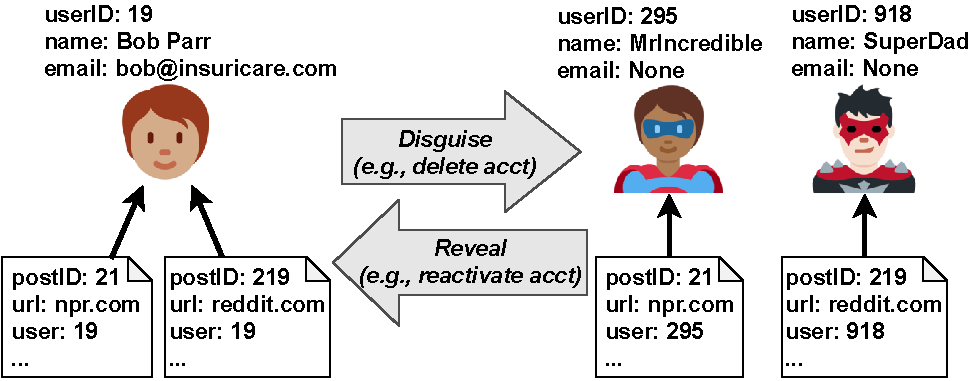
\includegraphics[width=0.5\textwidth]{img/disguises}

    \caption{Disguises move the target object (in this example, a user Bob) from an identity-revealing
    guise to privacy-preserving guises.}
    \label{fig:example}
\end{figure}
\fi

\begin{figure*}[t!]
    \centering
    \footnotesize
\begin{tabular}{@{}c|c|c|c@{}}
\textbf{User Transformation Spec} & \textbf{User Object} & \textbf{Guise 1} &
    \textbf{Guise 2} \\
\begin{lstlisting}[language=Rust]
"id":       IDAttribute,
"name":     Gen(Random),
"active":   Gen(Default(false)),
"darkmode": CopyAll,
"notifs":   CopyOnce+Gen(Default(false)),
"tag_id":   GenForeignKey,
\end{lstlisting}
    &
\begin{lstlisting}[language=Rust]
"id":       19,
"name":     BobParr,
"active":   true,
"darkmode": false,
"notifs":   true,
"tag_id":   11
\end{lstlisting}
&
\begin{lstlisting}[language=Rust]
"id":       295,
"name":     MrIncredible,
"active":   false,
"darkmode": false,
"notifs":   true,
"tag_id":   81483
\end{lstlisting}
&
\begin{lstlisting}[language=Rust]
"id":       918,
"name":     SuperDad,
"active":   false,
"darkmode": false,
"notifs":   false,
"tag_id":   15592
\end{lstlisting}
\end{tabular}
    \caption{Creating two guises of an example user (of a synthetic application schema).}
    \label{fig:guises}
\end{figure*}


The disguise specification must identify the following:
\begin{enumerate}
\item What data needs to be transformed to disguise Bob? 
\item How should the data be transformed to disguise Bob?
\item How can the disguise undo the transformations to reveal Bob if Bob ever returns?
\end{enumerate}

A data disguise is written once by the developer, and applied to all objects in the  
specific instance of the object graph.
%
The disguise specifies, for each object type, a set of conditions to filter out the objects to 
transform, and the transformation to be applied to these objects. These transformations can be
optionally archived to enable disguise reversal.
%that turn objects into one or more guises (or remove the object completely). 
%Developers specify disguises in two parts. The
%first specifies how to create guises of a given object type (\S\ref{sec:guises}). The second specifies in which
%contexts objects should be transformed into guises or removed (\S\ref{sec:context}).
%
A disguising tool then applies the disguise by first determining the current context of objects in the object
graph, and then applying the appropriate transformation for that context.
%\ie from what type of edge, and sensitivity context.

\subsection{Context-Specific Transformations}
\label{sec:context}

Developers specify \textbf{contexts}, and transformations to the objects that match each context. 
%
% SOURCE = CHILD
% DEST = PARENT
%
%In the following, we refer to edge types in the object graph, which have a \emph{source} object type and a \emph{destination} object type,
%where the source references the destination (\eg via a foreign key column in a relational database).
%
A context consists of an object type, and a set of \textbf{constraints} on the objects' attributes
(\S\ref{sec:constraints}).
Given an instance of the object graph, a set of objects in the graph
satisfy the context if the objects are of the specified object type and the objects'
attributes satisfy the constraints.

For each context, developers specify to either remove matching objects (which also removes all
descendents---objects that refer to these objects---as well), or to transform each object into
a single guise by specifying a \textbf{single-guise transformation}~(\S\ref{sec:single_guise}). 
Furthermore, to allow some matching objects to retain their original attribute values, 
developers can specify \textbf{thresholds} on attributes~(S\ref{sec:threshold}), transforming
only enough matching objects to achieve the threshold.

%
In the following, we assume that objects have identifier attributes (\eg \texttt{id} in Figure~\ref{fig:guises}); and
some attributes are reference attributes that form edges in the graph to referred objects (\eg
\texttt{tag\_id} is a foreign key constraint to tag objects).

\subsection{Object Attribute Constraints}
\label{sec:constraints} 

Object attribute constraints consist of (some conjunction) of the following constraints:
\begin{itemize}[nosep]
\item \textbf{Reference content} constraints on reference attributes are functions that
    take both the object and the referenced object as input, and return true or false. 
    %
    %For example, perhaps we want to decorrelate paper-tag edge \emph{only if} the tags were created by the user who is leaving.
\item \textbf{Value content} constraints on non-reference (value) attributes are functions that take the object as
input, and return true or false.  
\item \textbf{Sensitive reference} constraints on reference attributes match only objects that refer
    to sensitive objects (\ie connects back to the target object of the disguise).
\end{itemize}

\subsection{Single-Guise Transformations}
\label{sec:single_guise} 
Single-guise transformations are specified at attribute-level granularity. 
Guise identifier attributes are unique and random values. 
%
Other guise attributes either copy the original object attribute value, 
or transform the object attribute.  

If the attribute is a non-referencing, value attribute, the attribute transformation takes the
object attribute value as input, and generates a new guise value (\eg hashing the value, generating
random values, or setting the value to some default).  The guise attribute value can depend only on
the value of the object's attribute.

If the attribute is a reference attribute, the attribute transformation \textbf{decorrelates} the 
object from the reference. Decorrelation creates a new reference guise based on the referenced
object (\S\ref{sec:reference_guises}), and the guise's reference attribute will refer to the
created reference.

\subsection{Reference Guise Creation}
\label{sec:reference_guises} 
%
Decorrelating references requires creating guises for the referenced objects. One referenced object may turn into many
reference guises (one for each context-matching object that all should be decorrelated).  Because
multiple reference guises may be created to decorrelate objects from the reference object,
developers needs to specify how to transform the reference object into a guise \emph{for each guise
created}.

%
Developers specify \textbf{many-guise transformations} for each object type that may be a reference;
these transformations are \emph{independent} of any single context, because many-guise
transformations only occur for the purpose of decorrelation, and can occur in many contexts.
%
Figure~\ref{fig:guises} shows an example, producing guises for user objects.

A many-guise transformation for an object type consists of a single-guise transformation (as
described above, \ie copying or generating new object attributes); and additional per-attribute
annotations that specify whether the transformation should be applied to create all guises, or
applied to create all but $n$ guises. In the latter case, $n$ guises will simply copy the
object's attributes, and the other guises will transform the object's attributes according to the
single-guise transformation.

Note that creating reference object guises may also require recursively creating guises for references of
the reference object, using the (context-independent) many-guise transformation for those ancestral reference
object types.

\subsection{Partially Applying Context Transformations}
\label{sec:threshold} 

Developers may want to transform some attributes in only a subset of all context-matching objects when
changing them into guises. 
For example, let the context match only the papers written by the targeted user. These papers should
be decorrelated from a tag only enough to ensure that these sensitive papers comprise less than 10\%
of all papers with that tag. Importantly, papers falling below the 10\% threshold can retain the
reference to the tag.

To transform attributes in only a subset of context-matching objects, developers can associate a
\emph{threshold} with an attribute of the context's object type.  A threshold is defined as follows:

Consider all objects of the context's object type that share the same attribute value (\eg a
referenced tag, or location value). This set contains both context-matching objects, and objects
ouside the context. The threshold for the attribute determines the maximum proportion of these
objects that are context-matching, and whose attribute value should not be transformed when the
object becomes a guise.

All context-matching objects falling above the threshold transform the attribute according to the
associated attribute transformation, while all objects falling below the threshold leave the
attribute unchanged. 

In our paper-tag example, the developer specifies a threshold of 10\% for the tag reference
attribute: any sensitive papers falling below the 10\% threshold can retain their reference to the tag.

Thresholds can also be associated with a set of
attributes, for example determining the maximum proportion of papers referencing a particular tag
\emph{and} a particular location attribute value that can match the context.

\lyt{Similar to k-anonymity, we could have a term that looks at how many unique ``identities'' are
correlated with a particular attribute (rather than just how many objects share the same attribute);
this attribute is a quasi-identifier, and the objects of this type achieve $k$-anonymity if there
are at least $k$ objects with the same attribute?}

\lyt{l-diversity comes into play if \eg the paper timestamp is sensitive, and even if $k$ individuals have papers
with that tag, all papers have the same timestamp. We need many different timestamps for the same
$k$ individuals.}

\subsection{What Can Disguises Specify?}

\paragraph{Supported Privacy Transformations}

\paragraph{Out-of-Scope Privacy Transformations}

%-------------------------------------------------------------------------------
\subsection{Applying Data Disguises}
%-------------------------------------------------------------------------------
The data disguising tool applies the disguise to each group of objects with the same object type.

\paragraph{Considerations}
One problem the tool must solve is when to terminate disguise applications. For instance, what
should happen if disguise conditions always match some objects, and if the transformation
does not modify objects such that they no longer match the conditions?

Disguise application interleaves with normal query execution, resulting in eventually consistent
disguise application. This raises potential issues, since the underlying database may change during
disguise application, and cause conflicting changes or non-terminating disguise application.

\fi
